\chapter{Implementation} \label{chap:impl}

After having presented the proposed system architecture we will now move forward to describing how the project implementation was performed, starting with the evolution of the initial concept and then going through the hardware and software implementations.
After having done so, we will also explain the limitations and design choices that were known to limit the outcome, up to a certain degree.

These limitations were mainly due to lack of time to develop better alternatives as the entire project, to include such alternatives, would require more development time, or more developers working together on this project.
All of these were pondered and they were only left out or replaced by simpler versions after making sure they would only reduce user friendliness or not include advanced functionality not part of the scope of the original concept.
As the result of this project is intended to be a proof of concept, user friendliness was only an optional objetive, which eventually had to be left behind.

\section{Concept development}

In the beginning of this project, while being to clouded with the idea of applying the concept to a robotic system, we explored several possibilities of creating a demonstrator based on a robotic arm.
The conceptual idea was to preprogram a path on the robotic arm that had to be followed when its actuators were commanded through a real-time network.
One could define a 2D path on a sheet of paper and the robotic arm would have to follow it with a pen, drawing the travelled path.
This way, the effects of network cycle time would be indirectly visible when comparing the preprogrammed path and the actual travelled path.

This concept had an interesting potential but soon enough we came across a not so obvious problem: from the user's point of view, when looking at a robotic arm system, the attention would almost certainly go towards what the robotic arm could do instead of focusing on what was happening in the background, especially in terms of communications and how they affected the control system.

After deciding this was not the way to go, we performed a retrospection exercise and analysed what was good about this first idea and why we had it in the first place.
The underlying concept that made us consider this approach is that robotic systems are characterised by one traversal aspect: movement control.
In fact, wanting to demonstrate the effects of network cycle time in a control application, controlling movement seems to best fulfil the purpose.
This type of control requires short cycle times and deterministic periodicity, making it very susceptible to the effects of network cycle time.
Additionally, it provides the demonstrator with a graspable connection to reality.

The second iteration on the base concept led us to an idea still based on movement control but with a simpler approach: two perforated discs attached to motors, facing each other, would have their movement controlled independently.
One of the discs would have a control loop closed locally on the field device and the other one would have it closed on the master controller node, traversing a real-time Ethernet network.
With both discs coupled with a single string of spaghetti pasta, any effects the real-time Ethernet network would introduce on the control system would make the two discs' movement desynchronise and, as such, it would manifest through the spaghetti string breaking.
We decided not to pursue this idea further because we expected, from the beginning, that the effects introduced by the communication network would have a small impact on performance and that, in this case, the spaghetti string would possibly have enough elasticity to withstand the small expected position slippages between the two discs.

Given the reason for discarding the second concept, we decided the best way to visualise such small differences would be to compare data points relative to the movement of both the locally and remote controlled run times.
In order to generate such data, virtually any type of physical movement can be utilised.
So, simplifying the second concept iteration into a third one, the idea was now to control the movement of a single disc.
The control itself can still be performed both locally on the field device or remotely on the master device, but not simultaneously.
This way, one can create a sequence of set-points and pass them to both types of control which, in turn, will generate data relative to the disc's movement.
One can then compare these data sets by creating graphs or using any other relevant methods.


\subsection{Hardware} \label{sec:proposed-hardware}

While keeping a careful consideration of characteristics between options and maintaining the requirements in focus, hardware parts were chosen to build each section of the demonstrator.

\subsubsection{Master node}

Taking into account the two operation modes the demonstrator should have, we extrapolated that the master node must be able to perform numeric calculations and serve as an EtherCAT master device.
As the EtherCAT master implementation can be done using a generic Ethernet MAC interface card (refer to \ref{subsubsec:master_devices} for an explanation), everything the master node requires in term of hardware is a computational platform (computer, microcontroller, etc.) with access to a generic Ethernet MAC interface card.

As of today, most education facilities provide students with access to desktop computers.
For many years now, motherboard vendors have integrated Ethernet MAC interface cards into the motherboards themselves, as it has become the \emph{de facto} standard for Internet connectivity in desktop computers.

As such, we decided to implement the master device in a desktop computer in order to minimize costs and leverage the computational power modern computer systems possess.

\subsubsection{Slave node} \label{subsubsec:slave_hdw}

On the other hand, the slave node's hardware was harder to choose.
In order to implement the desired EtherCAT slave (see \ref{subsubsec:slave_devices}), one must be aware when choosing a computational platform to check the availability of a fitting ESC board and, simultaneously, the support for motor and encoder interfaces.

After some research, two options presented themselves as possible platforms for the slave device: an Arduino UNO or a Raspberry Pi.
ESC boards exist for both these platforms, as well as good support in terms of "shield boards" for motor interfaces.
In the end, we decided to go with a solution based on a Raspberry Pi, as it provides a more robust and versatile computing platform, especially considering the local control configuration, where position/velocity control algorithms will need to be executed on this platform.

The ESC board chosen for the Raspberry Pi was the Hilscher's \emph{netHAT 52-RTE} (see \url{www.netiot.com/interface/nethat}).
This board supports communication with three real-time Ethernet protocols (PROFINET, EtherNet/IP or EtherCAT), chosen with a simple firmware loading procedure.
It complies with the Hardware Attached on Top (HAT) specification for the Raspberry Pi (see \url{www.github.com/raspberrypi/hats}) and uses the \emph{SPI0} interface to communicate with it.
The board also includes the respective Electronic Data Sheet (EDS) files to be imported by the EtherCAT master, used to identify the characteristics and functionality of slaves implemented using this setup.

% Motor choice

With the intention to relieve the Raspberry Pi from having to generate the PWM signal to drive the motor, we included the DFRobot's DFR0592 board onto the design.
This board also complies with the HAT specification and communicates with the Raspberry Pi via the Inter-Integrated Circuit (I\textsuperscript{2}C or I2C) interface.
It provides interface with two DC motors and two incremental encoders, all managed by an STMicroelectronics's STM32 chip.
The motor interface also includes the necessary DC-motor driver chip, allowing direct connection of the motor's terminals and power supply to the board itself.

Initially we planed on using this board's incremental encoder interface to also relieve the Raspberry Pi from such task but, as our preliminary tests concluded, it only exports the Revolutions Per Minute (RPM) value extrapolated from the encoder's pulse count and not the pulse count itself.
Furthermore, the RPM value is only updated once every 100ms, which is to large of a period for motion control.

\begin{figure}[htp]
	\centering
	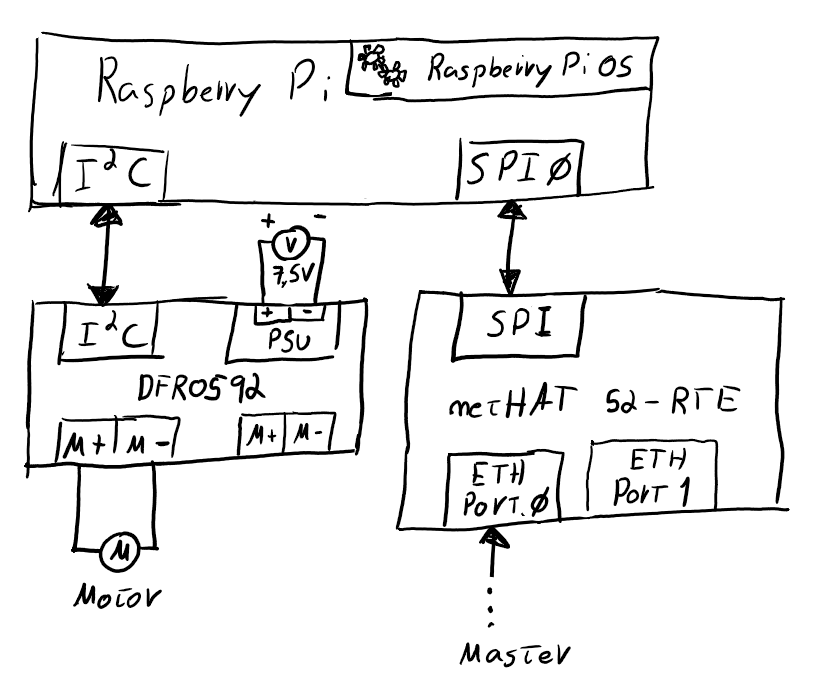
\includegraphics[width=1\textwidth]{slave_architecture.png}
	\caption{Graphical representation of the remote control scheme}
	\label{fig:slave_architecture}
\end{figure}\footnote{placeholder image}


\subsection{Software} \label{sec:proposed-software}

As can be expected, recent digital computing platforms require software to perform the necessary tasks.
As such, both the master node (computer) and the slave device (Raspberry Pi) will each require an Operating System (OS) to manage the execution of tasks.
The Raspberry Pi has a dedicated Linux OS called \emph{Raspberry Pi OS}, which is a fork from Debian (see \url{https://www.raspberrypi.org/software/}.
We will be using the Lite version of this OS for the Raspberry Pi as it is the easiest to setup and the most tested and stable OS for this platform.
Regarding the master node computer we will be using Microsoft's Windows 10 as the chosen OS, not only because most computers come pre-installed with it, but also because it is one of the few supported OSes by the CODESYS development application \cite{ide:codesys}, presented below.

\subsubsection{Master node software}

In order for us to create a control application on a generic computer, an appropriate software platform must be chosen.
Because we are working with industrial technology, a proper industrial control and automation software should be used.

CODESYS is a generic platform to develop industrial control and automation applications based on the IEC 61131-3 standard.
It includes support for hardware from multiple vendors as well as the ability to create a Software PLC (SoftPLC) from any generic computer hardware.
This platform makes the software editor available to use for free and allows control applications to run for two hours in demonstration/testing mode, uninterrupted.
This is a great option for development and testing purposes as only the final product with uninterrupted execution requirements for unknown periods of time will require a license to be purchased.
Additionally, CODESYS natively supports the most common industrial communication networks, including EtherCAT, meaning one can develop a device with communication capabilities with one or more of these networks.

With all this, we will use the CODESYS platform to create a SoftPLC to act as an EtherCAT master device for or demonstrator.
As we are looking forward to develop a proof-of-concept system, we don't require application runtimes larger than two hours.

Because we want to involve the end-user into the process of setting-up and running the experiments by themselves, we decided to leave the implementation of the master node's software to be dealt with by the end-user.
By doing such, we will also be indirectly expanding the set of conceptual experiments the demonstrator can handle by allowing anyone to implement their own ideas, as the slave device will always work the same way.

\subsubsection{Slave node software}

After having chosen the Hilscher's ESC HAT for the Raspberry Pi (see \ref{subsubsec:slave_hdw}), which will be running a Linux distribution, and decided to use the CODESYS platform for the master, we initially planned to also use CODESYS to program the slave device.
Although its editor is only designed to work under Windows, the SoftPLC runtime can run under Linux, with a version specifically targeting the Raspberry Pi platform.
Unfortunately, CODESYS doesn't support developing programs for EtherCAT slave devices, specifically, as these are usually programmed by manufacturers themselves and not by a system integrator or end-user.

Additionally, Hilscher only provides a library and accompanying API definitions for the C programming language, meaning at least the software module that needs to interact directly with the ESC will need to be programmed in C language.
As this is the most widely used programming language in the Linux universe, if during development we conclude we require some library to provide us with some advanced functionality, the probability of existing one for the C language is much higher than with less widespread languages.
As such, this is going to be our preferred programming language for implementing the EtherCAT's slave software running on the Raspberry Pi.




\section{Limitations} \label{sec:limitations}




\section{Summary} \label{sec:impl-summary}
This chapter focused almost exclusively on technical details of how the final solution was implemented.
Starting with the choice of hardware components, going through their assembly and then moving towards the complex and extensive software required to give the desired slave device all planned functionality.

Not only the good things have been explained but we have also expressed those we are aware could have been better implemented or designed.
Even though this project was developed during difficult times, especially from having been done entirely on a full-remote work basis, most of the things explained as weak spots were considered from the beginning.
Difficult times impose harder decisions and \emph{simplify} became the daily word of choice because, sometimes, \emph{less is much more}.
It's one thing to design simple systems, but it's a much harder thing to simplify complex systems and boil them down to their bare-bones.

